% Jane - FastSCSS single-best output, but is considerably faster by not maintaining separate model costs and by deleting recombined hypotheses
% Jane - not multithreaded
% Zens & Ney - don't compare different coverage config. Not focused on speed.
%
% File ACL2016.tex
%

\documentclass[11pt]{article}
\usepackage{acl2016}
\usepackage{times}
\usepackage{latexsym}
\usepackage{algorithmic}
\usepackage{graphicx}

%\aclfinalcopy % Uncomment this line for the final submission
%\def\aclpaperid{***} %  Enter the acl Paper ID here

% To expand the titlebox for more authors, uncomment
% below and set accordingly.
% \addtolength\titlebox{.5in}    

\newcommand\BibTeX{B{\sc ib}\TeX}


\title{Fast, Scalable Phrase-Based SMT Decoding}

\author{Hieu Hoang\\
	    Moses Machine Translation CIC\\
	    {\tt hieu@moses-mt.org}
	  \And
	Nicolay Bogoychev\\
  	University of Edinburgh\\
  	10 Crichton Street\\
  	Edinburgh, Scotland, EH10 9AB\\
  {\tt s1031254@sms.ed.ac.uk}
	  \And
	Lane Schwartz\\
  	University of Illinois\\
  {\tt lanes@illinois.edu}
	  \AND
	Kenneth Heafield\\
  	University of Edinburgh\\
  {\tt kheafiel@inf.ed.ac.uk}
	  \And
	Marcin Junczys-Dowmunt\\
	Faculty of Mathematics and Computer Science \\
	Adam Mickiewicz University\\
  {\tt junczys@amu.edu.pl}
	}
	
  
\date{}

\begin{document}

\maketitle

\begin{abstract}
The utilization of statistical machine translation (SMT) has grown enormously over the last decade, many using open-source software developed by the NLP community. As commercial use has increased, there is need that for the software to be optimized for their requirements, in particular, faster phrase-based decoding and more efficient utilization of modern multicore servers.

In this paper we re-examining the major components of phrase-based decoding and decoder implementation with particular emphasis on speed and scalability on multicore machines. The result is a drop-in replacement for the Moses decoder which is up to fifteen times faster and scales monotonically with the number of cores. 

\end{abstract}

\section{Introduction}

SMT has steadily progressed from a research discipline to commercial viability during the past decade as can be seen from services such as the Google and Microsoft Translation services. As well as general purpose services such as these, there is a large number of companies that offer customized translation systems, as well as  companies and organization that implement in-house solutions. Many of these customized solutions use Moses as their SMT engine.

For many users, decoding is the most time-critical part of the translation process. Making use of the multiple cores that are now ubiquitous in todays servers is a common strategy to ameliorate this issue. However, it has been noticed that the Moses decoder, amongst others, is unable to efficiently use multiple cores~\cite{mfernandez2016boosting}. That is, decoding speed does not substantially increase when more cores are used, in fact, it may actually \emph{decrease} when using more cores. There have been speculation on the causes of the inefficiency as well as potential remedies. 

This paper is the first we know of that focuses on improving decoding speed on multicore servers. We will take a holistic approach to solving this issue, re-implementing the decoder's structure to optimize for speed, re-assessing some of the optimization assumptions made in the implementation of significant parts of the decoder, as well as exploring changes to the core search algorithm. We will compare and contrast decoder implementations, not just decoding algorithms or individual components. 

We will present a phrase-based decoder that is significantly faster than the Moses baseline for single-threaded operation, and scales monotonically with the number of cores.

As far as possible, model scores and functionality are compatible with Moses to aid comparison and ease transition for existing users. All source code will be made available under an open-source license.

\subsection{Prior Work}

Most prior work on increasing decoding speed look to optimizing specific components of the decoder or the decoding algorithm. 

~\newcite{Heafield-kenlm} and ~\newcite{yasuhara-EtAl:2013:EMNLP} describes fast, efficient datastructures for language models. ~\newcite{zens2007efficient} describes an implementation of a phrase-table for an SMT decoder that is loaded on demand, reducing the initial loading time and memory requirements. ~\newcite{junczys_tsd_2012b} extends this by compressing the on-disk phrase table and lexicalized re-ordering model. 

~\newcite{Chiang:2007:cl} describes the cube-pruning and cube-growing algorithm which allows the tradeoff between speed and translation quality to the adjusted with a single parameter. ~\newcite{wuebker2012fast} note that language model querying is amongst the most expensive operation in decoding. They sought to improved decoding speed by caching score computations early pruning of translation options. This work is similar to ~\newcite{Heafield-mtplz} which group hypotheses with identical language model context and incrementally expand them, reducing LM querying.

~\newcite{mfernandez2016boosting} was concerned with multi-core speed but treat the decoding process as a black box within a parallelization framework.

There are a number of phrase-based decoding implementations, many of which implements the extensions to the phrase-based model described above.

The most well known is Moses~\cite{koehn-EtAl:2007:PosterDemo} which implements a number of speed optimizations, including cube-pruning. It is widely used for MT research and commercial use. 

Joshua~\cite{Joshua-Decoder} also supports cube-pruning for phrase-based models. Phrasal~\cite{spence2014phrasal} supports a number of variants of the phrase-based model. Jane~\cite{peitz2012jane} supports the language model look-ahead described in ~\newcite{wuebker2012fast} in addition to other tools to speed up decoding such as having a separate fast, lightweight decoder. mtplz is a specialized decoder developed to implement the incremental decoding described in ~\newcite{Heafield-mtplz}.

The Moses, Joshua and Phrasal decoders implement multithreading, however, they all report scalability problems, either in the paper (Phrasal) or via social media (Moses\footnote{\scriptsize https://github.com/moses-smt/mosesdecoder/issues/39} and Joshua\footnote{\scriptsize https://twitter.com/ApacheJoshua/status/342022794097340416}).

Jane and mtplz are single-threaded decoders, relying on external applications to parallelize operations. This has the advantage it is easier to parallelize processing across multiple servers, not just multiple cores. As we shall see, this method does not scale beyond a small number of cores when attempting to scale to multiple cores within one server.

This paper not only focuses faster single-threaded decoding but also on overcoming the shortcomings of existing decoding implementations on multicore servers.

The rest of the paper will be broken up into the following sections. Next, we will describe the phrase-based model and the major implementation components, with particular emphasis on decoding speed. We will then describe modifications to improve decoding speed and present results. We conclude in the last section and discuss future work.

\section{Phrase-Based Model}

The objective of decoding is to find the target translation with the maximum probability, given a source sentence. That is, for a source sentence $s$, the objective is to find a target translation $\hat{t}$ which has the highest conditional probability $p(t | s)$. Formally, this is written as:
\begin{equation}
\hat{t} = \arg \max_t p( t | s )
\label{eq:argmax-factored-trans}
\end{equation}
where the \emph{arg max} function is the search. The log-linear model generalizes Equation~\ref{eq:argmax-factored-trans} to include more component models and weighting each model according to the contribution of each model to the total probability. 
\begin{equation}
\label{eq:Log-Linear}
p(t | s) 	=  \frac{1}{Z} \exp ( \sum_m \lambda_m h_m ( t, s)^{} )
\end{equation}
where $\lambda_m$ is the weight, and $h_m$ is the feature function, or `score', for model $m$. $Z$ is the partition function which can be ignored for optimization. 

\subsection{Beam Search}

A translation of a source sentence is created by applying a series of translation rules which together translate each source word once, and only once. Each partial translation is known as a \emph{hypothesis}, which is created by applying a rule to an existing hypothesis. This \emph{hypothesis expansion} process starts with a hypothesis that has translated no source word and ends with completed hypotheses that have translated all source words. The highest-scoring completed hypothesis, according to the model score, is considered the best translation, $\hat{t} $.

In the phrase-based model, each rule translates a contiguous sequence of source words. Successive applications of translation rules do not have to be adjacent on the source side, depending on the distortion limit. The target output is constructed strictly left-to-right from the target side from the series of translation rules. 

A beam search algorithm is used to create the completed hypothesis set efficiently. Partial translations are organized into stacks where each stack holds a number of comparable hypotheses. Most phrase-based implementations place hypotheses in the same stack that have the same coverage cardinality $|C|$, where $C$ is  the coverage set, $C \subseteq \{1,2,... |s| \} $ of the number of  source words translated. 

\subsection{Feature Functions}

Features functions are the $h_m$ in Equation~\ref{eq:Log-Linear}, calculating a score for each hypothesis.

The standard feature functions in the phrase-based model include:
\begin{enumerate}
  \item \vspace{-2 mm} a distortion penalty
  \item \vspace{-2 mm} a phrase-penalty,
  \item \vspace{-2 mm} a word penalty,
  \item \vspace{-2 mm} an unknown word penalty.
  \item \vspace{-2 mm} log transforms of the target language model probability $p(t)$, 
  \item \vspace{-2 mm} log transforms translation model probabilities, $p_{TM}(t|s) $ and $p_{TM}(s|t)$, and word-based translation probabilities $p_w(t|s)$ and $p_w(s|t)$,
  \item \vspace{-2 mm} log transforms of the lexicalized re-ordering probabilities,
\end{enumerate}
%which we have suffixed with $_{TM} $ to avoid confusion with the overall model probability $ p(t|s) $ and $ p(s|t)$. 

Of these feature functions, the first four are simple and do not leave much room for optimization. As have already been mentioned, the language model consumes a large part of decoding time but it has already been heavily optimized in previous works such as ~\newcite{Heafield-kenlm} and ~\newcite{yasuhara-EtAl:2013:EMNLP}.

Therefore, we will focus on optimizing only the phrase-table and lexicalized reordering model.

\section{Proposed Improvements}

Apart from the two feature function optimization detailed in the last section, we will investigate two other optimizations, all described below.

\subsection{Efficient Memory Allocation}

The search algorithm creates and destroy a large number of hypothesis and related objects. The memory allocation required puts a burden on the operating system due to the need to synchronize  memory access. This problem worsens with multi-threaded applications such as Moses.

Libraries such as tcmalloc~\cite{ghemawat2009tcmalloc} are designed to reduce locking contention for multi-threaded application but in our case, this is still not enough. 

We shall seek to improve decoding speed by replacing the operating system's general purpose memory management with our own custom memory management scheme. In time-critical parts of the decoder, memory will be allocated from a memory pool. 

A memory pool is a large block of memory that has been pre-allocated by the operating system from which smaller blocks can be give out to the application. We will use a thread-specific memory pools to avoid locking contention during memory access. Our memory pool will be dynamic, growing in size when required but never reducing in size.

To further increase memory management speed, objects are not deleted, instead the memory pool is simply reset and reused for each input sentence. This can result in high memory usage so object queues are available for high-churn objects which allows the decoder to re-use portion of the memory pool before it is reset. The object queues are LIFO so that recently accessed memory are used, increasing CPU cache hits.

%The speed of memory access is dependent on whether the data is in the CPU cache which is a constrained resource compared to memory size, typically 20MB in the latest processors. We shall seek to re-use recently accessed information to increase likelihood of the data being in the CPU cache. 

%In multiprocessor servers, the CPU cache is attached to each processor and each core. If a sentences is being decoded on one CPU is switched to another, the CPU cache on the new CPU must be repopulated, slowing down decoding. We will therefore investigate binding threads to specific cores.

\subsection{Stack Configurations}

The most popular stack configuration for phrase-based model, as implemented in Pharaoh, Moses and Joshua, is coverage cardinality, that is, hypotheses that have translated the same number of source words are stored in the same stack. Since stack pruning occurs in each stack independently of each other, this affect the decoder's search errors.

However, there are alternatives to the coverage cardinality configuration. ~\newcite{Och:2001a} uses a single stack for all hypotheses, ~\newcite{Brown:1993} uses coverage stacks (ie. one stack per unique coverage vector) while ~\newcite{peitz2012jane} and ~\newcite{Zens+Ney:2008:iwslt} apply both coverage and cardinality pruning. While useful, these prior works present only one particular stack configuration each.

~\newcite{ortizmartinez-garciavarea-casacuberta:2006:WMT} explore a range of stack configurations by defining a granularity parameter which controls the maximum number of stacks required to decode a sentence. 

We shall re-visit the question of stack configuration with a particular emphasis on how they can help improve the tradeoff between speed and translation quality. We will do so in the context of the cube-pruning algorithm, the algorithm that we will be using and which was not available to many of the earlier work.

\subsection{Phrase-Table Optimizations}

For any phrase-table table of a realistic size, memory and loading time constraints requires us to use load-on-demand implementations of which Moses can make use of, each with differing performance characteristics. Figure~\ref{fig:moses-phrase-tables-time} shows the time taken to decode 800,000 sentences for the fastest two implementations.
\begin{figure}[h]
\centering
\begin{tabular}{cc}
{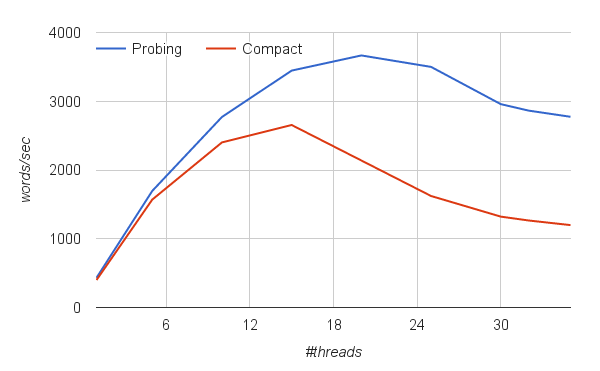
\includegraphics[scale=0.4]{moses-phrase-table.png}} 
\end{tabular}
\caption{Moses decoding time with two different phrase-table implementations}
\label{fig:moses-phrase-tables-time}
\end{figure} 
From this, it appears that the Probing phrase-table~\cite{Bogoychev:Thesis:2013} has the fastest translation rule lookup, especially with large number of cores, therefore, we will concentrate exclusively on this implementation from hereon.

We propose two optimizations. Firstly, the default translation rule caching mechanism in Moses saves the most recently used rules. However, this require locking and periodic clearing of old rules in order to reduce memory consumption resulting in \emph{slower} decoding, Table~\ref{tab:phrase-table-cache}. 
\begin{table}[h]
\small
\begin{center}
\begin{tabular}{|l|c|c|} \hline
		& No cache	& Caching \\ \hline
Decoding time  	& 2032 		& 2302 (+13\%) \\ \hline
\end{tabular}
\end{center}
\caption{Decoding time (in sec with 32 threads) when using phrase-table cache}
\label{tab:phrase-table-cache}
\end{table}

We shall explore a simpler caching mechanism that creates a static cache at the start of decoding of the most likely translation rules to be used.

Secondly, the Probing phrase-table use a simple compression algorithm to compress the target side of the translation rule. Compression was championed by ~\newcite{junczys_tsd_2012b} as the main reason behind the speed of their phrase-table but as we saw in Figure~\ref{fig:moses-phrase-tables-time}, this comes at the cost of scalability to large number of threads. We shall therefore take the opposite approach to and explore optimizing decoding speed by disabling compression.

\subsection{Lexicalized Reordering Model Optimizations}

Similar to the phrase-table, the lexicalized reordering model is trained on parallel data. A resultant model file is created in training which is then queried during decoding. Inevitably, the querying results in loss of decoding speed. Previous work such as~\newcite{junczys_tsd_2012b} improve querying speed with more efficient data structures.

However, the model's query keys are the source and target phrase of each translation rule. Rather than storing the lexicalized reordering model separately, we shall integrating it into the translation model, eliminating the need to query a separate file. This has precedent in ~\newcite{peitz2012jane} but the effect on decoding speed were not published. We will compare results with using a separate model in this paper.

\section{Experimental Setup}

We trained a phrase-based system using the Moses toolkit with standard settings. The training data consisted of most of the publicly available Arabic-English data from Opus~\cite{tiedemann2012parallel} containing over 69 million parallel sentences, and tuned on a held out set. The phrase-table was then pruned, keeping only the top 100 entries per source phrase, according to $p(t|s)$. All model files were then binarized; the language models were binarized using KenLM~\cite{Heafield-kenlm}, the phrase table using the Probing phrase-table, lexicalized reordering model using the compact data structure. These binary formats were chosen for their best-in-class multithreaded performance. Table~\ref{tab:model-files} gives details of the resultant sizes of the model files. For testing decoding speed, we used a subset of the training data, Table~\ref{tab:test-sets}. 
\begin{table}[h]
\begin{center}
\begin{tabular}{|l|c|c|} \hline
		& ar-en	& fr-en \\ \hline
Phrase table  	& 17 	& 5.8 \\
Language model 	& 3.1  	& 1.8 \\ 
Lex re. model	& 2.3	& 637MB \\ \hline
\end{tabular}
\end{center}
\caption{Model sizes in GB}
\label{tab:model-files}
\end{table}

For verification with a different dataset, we also used a second system trained on the French-English Europarl corpus (2m parallel sentences). The two different systems have characterics that we are interested in analyzing; ar-en have short sentences with large models while fr-en have overly long sentences with smaller models. Where we need to compare model scores, we used held out test sets.

\begin{table}[h]
\begin{center}
\small
\begin{tabular}{|l|r|r|} \hline
		& ar-en		& fr-en \\ \hline
\multicolumn{3}{|l|}{For speed testing} \\ \hline
Set name	& \multicolumn{2}{|c|}{Subset of training data} \\
\# sentences  	& 800k 		& 200k \\
\# words 	& 5.8m 		& 5.9m \\ 
Avg words/sent	& 7.3		& 29.7 \\ \hline
\multicolumn{3}{|l|}{For model score testing} \\ \hline
Set name	& OpenSubtitles	& newstest2011 \\
\# sentences  	& 2000 		& 3003 \\
\# words 	& 14,620 	& 86,162 \\ 
Avg words/sent	& 7.3		& 28.7 \\ \hline
\end{tabular}
\end{center}
\caption{Test sets}
\label{tab:test-sets}
\end{table}

Standard Moses phrase-based configurations are used, except that we use the cube-pruning algorithm~\cite{Chiang:2007:cl} with a pop-limit of 400, rather than the basic phrase-based algorithm. The cube-pruning algorithm is often employed by users who require fast decoding as it gives them the ability to trade speed with translation quality via a simple pop-limit parameter.

As a baseline, we use a recent\footnote{between January and May 2016} version of the Moses decoder taken from the github repository.

For all experiments, we used a Dell PowerEdge R620 server with 16 cores, 32 hyper-threads, split over 2 physical processors (Intel Xeon E5-2650 @ 2.00GHz). The server has 380GB RAM. The operating system was Ubuntu 14.04, the code was compiled with gcc 4.8.4 and Boost 1.59\footnote{http://boost.org/} and the tcmalloc library.

\section{Results}

\subsection{Optimizing Memory}

We instantiate two memory pools per decoding thread, one which is never reset and another which is reset after the decoding of each sentence. Data structures are created in either pool according to their life cycle.

Hypothesis objects and the data structures it contains are re-used by maintaining a thread-specific LIFO queue of unused, recombined and pruned objects from which new hypotheses are allocated in preference to create new hypotheses in the memory pool.

Each sentence is decoded from start to finish using one worker thread. The CPU affinity of each thread is set to a specific core to minimize memory page faults as a result of threads switching cores.

As can be seen in Table~\ref{tab:optimizing-memory}, over 24\% of the Moses decoder running time is spent on memory management and this increases to 39\% when 32 threads are used, dampening the scalability of the decoder. By contrast, our decoder spends 11\% on memory management and does not significantly increase with more threads.
\begin{table}[h]
\begin{center}
\small
\begin{tabular}{|l|c|c|c|c|} \hline
		& \multicolumn{2}{c|} {Moses}	& \multicolumn{2}{c|} {Our Work} \\ \hline
\# threads	& 1 		& 32	& 1 		& 32  \\ \hline
Memory  	& 24\%		& 39\% 	& 11\%		& 13\% \\
LM 		& 12\%	 	& 2\% 	& 47\%		& 38\% \\ 
Phrase-table	& 9\%	 	& 5\% 	& 2\%		& 4\% \\ 
Lex RO 		& 8\%	 	& 2\% 	& 2\%		& 2\% \\ 
Search 		& 2\%	 	& 0\% 	& 14\%		& 19\% \\ 
Misc/Unknown	& 45\%	 	& 39\% 	& 24\%		& 29\% \\ \hline
\end{tabular}
\end{center}
\caption{Profile of \%age decoding time}
\label{tab:optimizing-memory}
\end{table}

Figure~\ref{fig:mempool} compares the decoding time for Moses and our decoder, using the same models, parameters and test set. Our decoder is over 3 times faster with one thread, and 4.7 times faster using all cores. Like Moses, performance actually worsens after approximately 15 threads, however, the problem is not as pronounced. This gives us a better foundation on which to build further innovations for fast, multi-core decoding.
\begin{figure}[h]
\centering
\begin{tabular}{cc}
{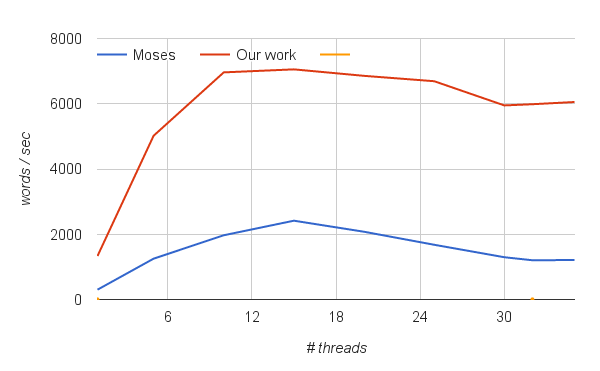
\includegraphics[scale=0.4]{mempool.png}} 
\end{tabular}
\caption{Decoding time of Moses and our decoder, using the same models}
\label{fig:mempool}
\end{figure} 

% A potential disadvantage of using memory pool is that the decoder will use more memory, however, Table~\ref{tab:memory-usage} shows that peak memory consumption are comparable.
% \begin{table}[h]
% \begin{center}
% \begin{tabular}{|l|c|c|} \hline
% 		& 1 thread	& 32 threads \\ \hline
% Moses  		& ???	 	& ??? \\
% Our work 	& ??? 		& ??? \\ \hline
% \end{tabular}
% \end{center}
% \caption{Peak Memory Usage in GB}
% \label{tab:memory-usage}
% \end{table}

\subsection{Stack Configuration}

We also note that the distortion limit which constrains hypothesis extension is dependent on the hypothesis' coverage vector, $C$ \emph{and} the end position of most recent source word that has been translated, $e$. The distortion limit must be checked for every instance of a hypothesis and translation rule, Figure~\ref{algo:Hypothesis Expansion with Unsorted Stack}.
\begin{figure} [h]
\begin{algorithmic}
%\REQUIRE source sentence $s$, translation options
\FORALL{ $hypo$ in $stack_{|C|}$} 
  \FORALL{ translation rules}
      \IF {can-expand($C(hypo)$, $e(hypo)$, translation rule range)}
	\STATE expand hypo with translation rule $\rightarrow$ new hypo
	\STATE add new hypo to next stack
      \ENDIF
  \ENDFOR % { translation options}
\ENDFOR % { hypothesis in $stack_i$} 
\end{algorithmic}
\caption{Hypothesis Expansion with Cardinality Stacks}
\label{algo:Hypothesis Expansion with Unsorted Stack}
\end{figure}
However, by separating hypotheses into set of hypotheses (\emph{'ministacks'}) according to coverage and end position, the distortion limit only needs to be checked for each ministack, Figure~\ref{algo:Hypothesis Expansion with Sorted Stack}. Furthermore, stack pruning is done on each of these hypotheses set therefore, changing how hypotheses are grouped can affect model scores. 
\begin{figure} [h]
\begin{algorithmic}
%\REQUIRE source sentence $s$, translation options
\FORALL{ $ministack_{C, e}$ in $stack_{|C|}$} 
  \FORALL{ translation rules}
    \IF {can-expand($C$, $e$, translation rule range)}
      \FORALL{ $hypo$ in $ministack_{C, e}$} 
	\STATE expand hypo with translation rule $\rightarrow$ new hypo
	\STATE add new hypo to next ministack
      \ENDFOR
    \ENDIF
  \ENDFOR % { translation options}
\ENDFOR % { hypothesis in $stack_i$} 
\end{algorithmic}
\caption{Hypothesis Expansion with Coverage \& End Position Stacks}
\label{algo:Hypothesis Expansion with Sorted Stack}
\end{figure}
We therefore looked at the effects of three stack configurations:
\begin{enumerate}
  \item \vspace{-2 mm} coverage cardinality,
  \item \vspace{-2 mm} coverage,
  \item \vspace{-2 mm} coverage and end position of most recent translated source word.
\end{enumerate}
Table~\ref{tab:stack-configuration} and Figure~\ref{fig:stack-configuration} present the tradeoff between decoding time and average model at various pop-limits.
\begin{table*}[t]
\small
\begin{center}
\begin{tabular}{|r|r|r|r|r|r|r|} \hline
Pop-limit	& \multicolumn{2}{c|}{Cardinality}	& \multicolumn{2}{c|}{Coverage}	& \multicolumn{2}{c|}{Coverage \& end pos} \\ \hline
		& Time		& Score			& Time		& Score		& Time		& Score	\\ \hline
100  		& 73		& -8.64513 		& 75		& -8.64513	& 72	& -8.64513 \\
500		& 237		& -8.59563		& 225		& -8.59563 	& 229	& -8.59612 \\
1,000	 	& 416		& -8.58700		& 397		& -8.58700	& 423	& -8.58700 \\ 
5,000 		& 1930		& -8.58165		& 1931		& -8.58165	& 2153	& -8.58098 \\ 
10,000 		& 3619		& -8.58133		& 3630		& -8.58133	& 4576	& -8.58015 \\ 
15,000 		& 4830		& -8.58130		& 5001		& -8.58130	& 7156	& -8.57999 \\ 
20,000 		& 5849		& -8.58130		& 5916		& -8.58130	& 9583	& -8.57994 \\ \hline
\end{tabular}
\end{center}
\caption{Decoding time (in secs with 32 threads) and average model scores for different stack configurations}
\label{tab:stack-configuration}
\end{table*}

\begin{figure}[h]
\centering
\begin{tabular}{cc}
{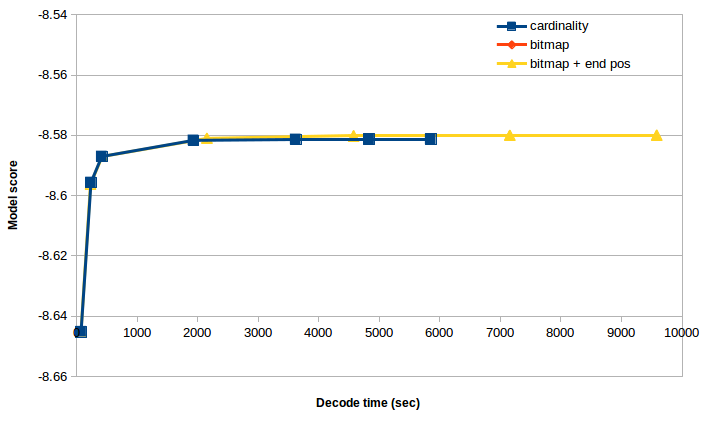
\includegraphics[scale=0.4]{stack-configuration.png}} 
\end{tabular}
\caption{Trade-off between decoding time average model scores for different stack configurations}
\label{fig:stack-configuration}
\end{figure} 
As can be seen, the model scores for all stack configurations are identical for low pop-limits parameters but grouping hypotheses into coverage \& end position produces higher model scores for higher pop-limits. It is also slower but the time/quality tradeoff is better overall with this stack configuration. For lower pop-limits this configuration is slightly slower but not by much. %, therefore, we shall stick with this Configuration for the remainder of the paper.

%Also, the cube-pruning algorithm contain a priority queue per set of hypotheses sets. This can be independent of how hypotheses are grouped. In the Moses implementation, the priority queue is also attached to the coverage cardinality, Figure~\ref{algo:Cube Pruning with Unsorted Stack}.
%\begin{figure} [h]
%\begin{algorithmic}
%%\REQUIRE source sentence $s$, translation options
%\STATE initialize $queue_{|C|}$
%\FOR{1 to pop-limit}
%  \STATE get best $item$ in $queue_{|C|}$
%  \STATE create hypo from $item$, coverage $C_{new}$
%  \STATE add hypo to $stack_{|C_{new}|}$
%  \STATE create next $items$
%  \STATE add new $items$ to $queue_{|C|}$
%\ENDFOR % { hypothesis in $stack_i$} 
%\end{algorithmic}
%\caption{Cube Pruning with Cardinality Stacks}
%\label{algo:Cube Pruning with Unsorted Stack}
%\end{figure}
%Again, we experiment with diffirent queue configurations, having separate queues for each cardinality, coverage, and coverage \& end position. The stack configuration remained constant (coverage \& end position with pop-limit of 400).
%\begin{table}[h]
%\small
%\begin{center}
%\begin{tabular}{|r|r|r|} \hline
%Queue configuration		& Time		& Score \\ \hline
%Cardinality			& 192		& -8.59922 \\
%Coverage			& 2,413		& -8.58635 \\
%Coverage \& end position	& 7,472		& -8.58263 \\ \hline
%\end{tabular}
%\end{center}
%\caption{Decoding time (in secs with 32 threads) and average model scores for different queue configurations}
%\label{tab:queue-configuration}
%\end{table}
%From the results in Table~\ref{tab:queue-configuration}, using finer grain queues does results in better model scores but it is significantly slower to decode.
%

\subsection{Translation Model}

The Moses translation model caches the most recently queried translation rules for later re-use. This has been shown to perform badly for fast phrase-tables such as those described by~\cite{Bogoychev:Thesis:2013}. We explore a simple caching mechanism that populates the cache during loading with rules that translates the most common source phrases. 
\begin{table}[h]
\small
\begin{center}
\begin{tabular}{|r|r|r|} \hline
Cache size	& Decoding Time & Cache Hit \%age	\\ \hline
Before caching	& 229	& N/A	 \\
0		& 239 (+4.4\%)	& 0\% \\
1,000		& 213 (-7.0\%)	& 11\% \\
2,000		& 204 (-10.9\%)	& 13\% \\
4,000		& 205 (-10.5\%)	& 14\% \\
10,000		& 207 (-9.7\%)	& 17\% \\ \hline
\end{tabular}
\end{center}
\caption{Decoding time (in secs with 32 threads) for varying cache sizes}
\label{tab:cache}
\end{table}
The static cache does not require the overhead of managing the most recently queried lookups but there is still some overhead in using a cache. Overall however, there was over a 10\% decrease in decoding time using the optimum cache size, Table~\ref{tab:cache}.

In the second optimization, we disable the compression. This increase the size of the binary files from 17GB to 23GB but the time saved not needing to decompress the data resulted in a 1.5\% decrease in decoding time with 1 thread and nearly 7\% when the CPUs are saturated, Table~\ref{tab:compression}.
\begin{table}[h]
\small
\begin{center}
\begin{tabular}{|r|r|r|} \hline
\# threads	& Compressed pt & Non-compressed pt \\ \hline
1		& 3052	& 3006 (-1.5\%) \\
5		& 756	& 644 (-14.8\%) \\
10		& 372	& 362 (-2.7\%) \\
15		& 284	& 250 (-12.0\%) \\
20		& 244	& 227 (-7.0\%) \\
25		& 218	& 209 (-4.1\%) \\
30		& 206	& 192 (-6.8\%) \\
35		& 203	& 189 (-6.9\%) \\ \hline
\end{tabular}
\end{center}
\caption{Decoding time (in secs with 32 threads) for compressed and non-compressed phrase-tables}
\label{tab:compression}
\end{table}

\subsection{Lexicalized Reordering Model}

The lexicalized reordering model assign a probability to a translation rule, given the relative ordering of the rule in the hypothesis. 

We integrate the lexicalized model file into the translation model but storing the model's probabilities in the phrase-table. This resulted in a significant decrease in decoding time, especially with high number of cores, Figure~\ref{fig:lex-ro}. 
\begin{figure}[h]
\centering
\begin{tabular}{cc}
{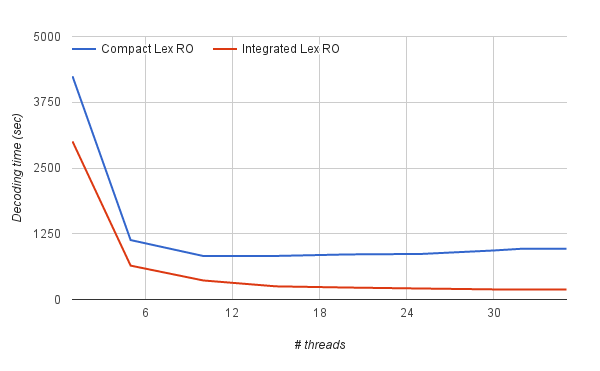
\includegraphics[scale=0.4]{lex-ro.png}} 
\end{tabular}
\caption{Decoding time with Compact Lexicalized Reordering, and integrated into a model the phrase-table}
\label{fig:lex-ro}
\end{figure} 
Integrating the lexicalized reordering model into the translation model decreases decoding time by 29\% with a single core but it is over 5 times faster using all cores. In fact, the decoding time with the integrated model is similar to that \emph{without} a lexilized reordering model. Critically for systems with multicores servers, it enables the decoder to continue to scale, making efficient use of all available cores. This is in contrast to using a separate lexicalized reordering model where decoding time flatten out and actually worsens after approximately 15 threads.

\subsection{Scalability}

\begin{figure}[h]
\centering
\begin{tabular}{cc}
{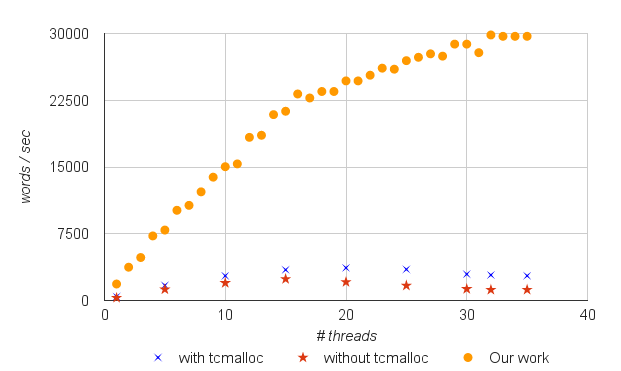
\includegraphics[scale=0.4]{scalability.png}} 
\end{tabular}
\caption{Our decoder's decoding speed}
\label{fig:speed}
\end{figure} 

Figure~\ref{fig:speed} shows decoding speed against the number of threads, measured in words translated per second. There is a constant increase in decoding speed when more threads are used, only decreasing slightly after 16 threads when hyperthreads are used. Overall, decoding is 12.5 times faster than single-threaded decoding when all 16 cores (32 hyperthreads) are fully utilized.

%Since the test server only has 16 real cores, additional threads must be run on the same physical cores as existing threads. This further constrains the resources that each thread has, therefore we see a markedly lower speed increase with each additional thread once there are more than 16 concurrent threads.

Overall though, the scalability is remarkably good, the decoder is able to make full use of all real and virtual cores. When all 16 cores are saturated with 2 hyper-thread each, the decoder is 16 times faster than single-threaded decoding. It is also 4.5 times faster than Moses with a single-thread and 9.6 faster when all cores are used.

This contrast with Moses where speed increases to approximately 16 threads but then actually become slower thereafter, Figure~\ref{fig:moses-speed}.
\begin{figure}[h]
\centering
\begin{tabular}{cc}
{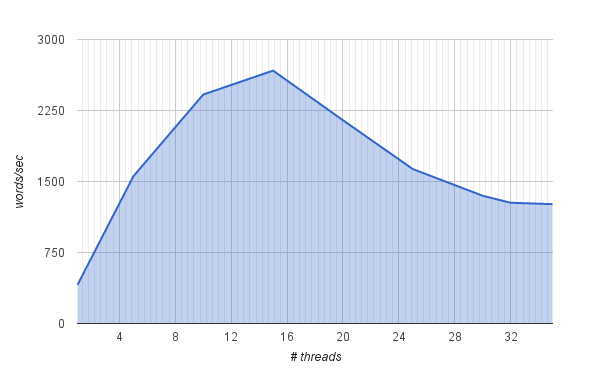
\includegraphics[scale=0.4]{moses-scalability.png}} 
\end{tabular}
\caption{Moses' decoding speed}
\label{fig:moses-speed}
\end{figure} 


\section{Other Models and Even More Cores}

Our decoder show no scalability issues when we tested with the same model and tested set on a larger server, Figure~\ref{fig:more-cores}.
\begin{figure}[h]
\centering
\begin{tabular}{cc}
{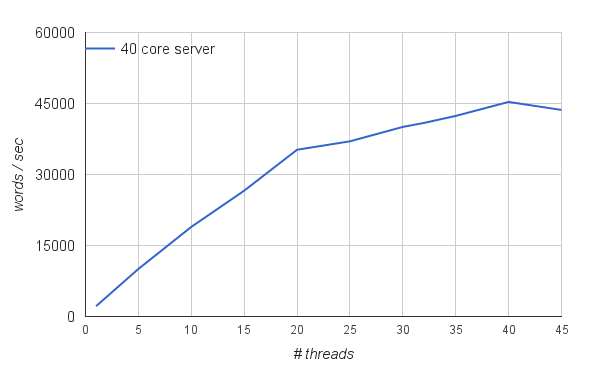
\includegraphics[scale=0.4]{more-cores.png}} 
\end{tabular}
\caption{Decoding speed for with bigger servers}
\label{fig:more-cores}
\end{figure} 

We verify the results with the French-English phrase-based system and test set. The speed gains are even greater than the Arabic-English test scenario, Figure~\ref{fig:fr-en-speed}. Our decoder is 5.4 times faster than Moses with a single-thread and 14.5 faster when all cores are saturated.
\begin{figure}[h]
\centering
\begin{tabular}{cc}
{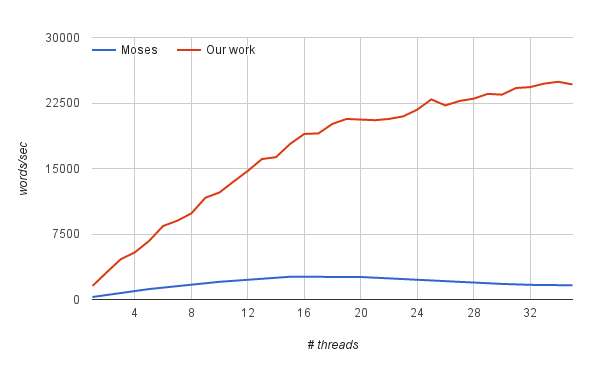
\includegraphics[scale=0.4]{fr-en-speed.png}} 
\end{tabular}
\caption{Decoding speed for fr-en model}
\label{fig:fr-en-speed}
\end{figure} 

\section{Conclusion}

We have presented a new decoder that is compatible with Moses. By studying the shortcomings of the current implementation, we are able to optimize for speed, particularly for multicore operation. This resulted in double digit gains compared to Moses on the same hardware. Our implementation is also unaffected by scalability issues that has afflicted Moses. % and continue to scale well for all possible cores we have tested it on.

In future, we shall investigate other major components of the decoding algorithm, particularly the language model which has not been touched in this paper. We shall also explore the underlying reasons for the scalability issues in Moses to get a better understanding where potential performance issues can arise. This has application to other algorithms beside MT decoding. 

% \section*{Acknowledgments}
% 
% Do not number the acknowledgment section.
% This section should not be presented for the submission version.

\bibliography{acl2016,mt,more}
\bibliographystyle{acl2016}


\end{document}
